%===============================================================================
% $Id: ifacconf.tex 19 2011-10-27 09:32:13Z jpuente $  
% Template for IFAC meeting papers
% Copyright (c) 2007-2008 International Federation of Automatic Control
%===============================================================================
\documentclass{ifacconf}

\usepackage{graphicx}      % include this line if your document contains figures
\usepackage{natbib}        % required for bibliography
%===============================================================================
\begin{document}
\begin{frontmatter}

\title{Force-Limited Control of Wave Energy Converters using a Describing Function Linearization\thanksref{footnoteinfo}} 
% Title, preferably not more than 10 words.

\thanks[footnoteinfo]{This material is based upon work supported by the National Science Foundation Graduate Research Fellowship under Grant No. DGE–2139899.}

\author[First]{Rebecca McCabe} 
\author[Second]{Maha N. Haji} 

\address*{Sibley School of Mechanical and Aerospace Engineering, Cornell University, 
   Ithaca, NY 14853 USA }
   \address[First]{e-mail: rgm222@cornell.edu}
   \address[Second]{e-mail: maha@cornell.edu}

\begin{abstract}                % Abstract of not more than 250 words.
Actuator saturation is a common nonlinearity in physical systems. In wave energy conversion, force saturation can be a convenient way to limit the size and cost of the generator and the mechanical loading on the drivetrain with minimal impact on energy generation. However, such nonlinear dynamics typically demand time-domain simulation rather than frequency-domain analysis, which increases computational cost and diminishes designer intuition. This paper proposes the use of describing functions to accurately linearize the force saturation dynamics and stay in the frequency domain. It explores the impact of the force limit on electrical power production of a generic single-body wave energy converter under energy-maximizing reactive control. A sweep of nondimensional coefficients is carried out to visualize the effect of the maximum force value on devices with different hydrodynamics and powertrain dynamics. Sensitivity results are discussed in the context of sizing drivetrain components such as the generator. The describing function method is over 200 times faster than a time-domain simulation and X times faster than a spectral-domain simulation, showing promise as a technique to enable future studies such as large-scale design optimization and control co-design.
\end{abstract}

\begin{keyword}
Constrained control, control of renewable energy resources, systems with saturation, nonlinear and optimal marine system control, sensors and actuators.
\end{keyword}

\end{frontmatter}
%===============================================================================

\section{Introduction}
Final page limit is 6, initial submissions can be 8 pages

Motivation

Lit review about force saturation in WECs

\section{Peak Limiting in the Linear Case}
\subsection{General Impedance-Matched System}
The analysis starts with a generic linear system modeled as a Thévenin equivalent circuit with AC voltage source $V_{th}$ and complex source impedance $Z_{th}$. The load impedance $Z_L$ is to be selected, with the conflicting goals of maximizing power transfer and minimizing the peak amplitude of load current or voltage, $I_L$ and $V_L$. Maximum power transfer occurs at $Z_L = Z_{th}^*$ where $*$ indicates the complex conjugate, minimum current at $Z_L \rightarrow \infty$, and minimum voltage at $Z_L = 0$.

See  Fig.~\ref{fig:circuit} for an example.

\begin{figure}
\begin{center}
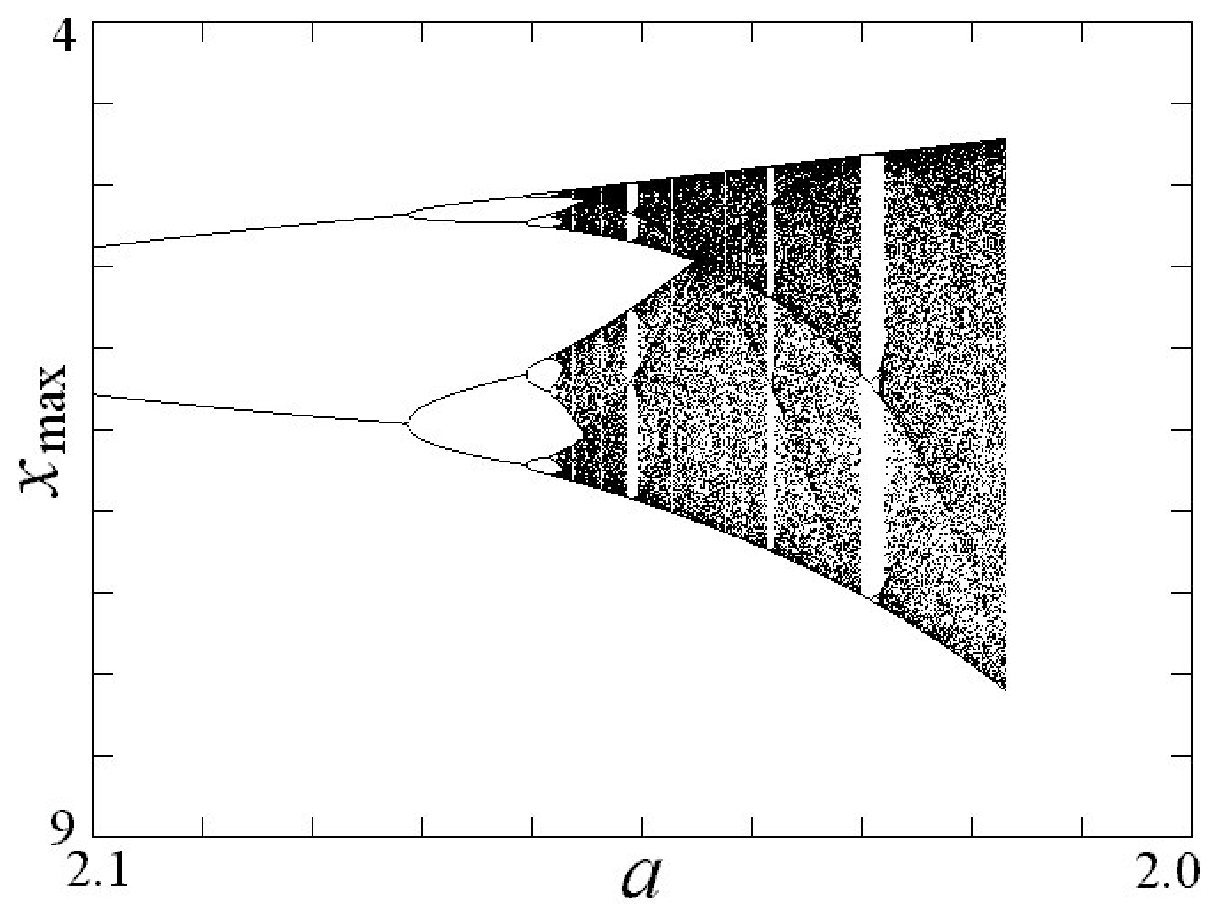
\includegraphics[width=8.4cm]{bifurcation}    % The printed column width is 8.4 cm.
\caption{Bifurcation: Plot of local maxima of $x$ with damping $a$ decreasing} 
\label{fig:circuit}
\end{center}
\end{figure}

\subsection{Wave Energy Converters}

\section{Saturation Nonlinearities and Describing Functions}

\subsection{Theory}

\subsection{Error Analysis}

\section{Sensitivities}
\subsection{Nondimensional Results}
\subsection{Dimensional Generator Sizing Implications}


See \cite{Abl:56}, \cite{AbTaRu:54}, \cite{Keo:58} and \cite{Pow:85}.

%% There are a number of predefined theorem-like environments in
%% ifacconf.cls:
%%
%% \begin{thm} ... \end{thm}            % Theorem
%% \begin{lem} ... \end{lem}            % Lemma
%% \begin{claim} ... \end{claim}        % Claim
%% \begin{conj} ... \end{conj}          % Conjecture
%% \begin{cor} ... \end{cor}            % Corollary
%% \begin{fact} ... \end{fact}          % Fact
%% \begin{hypo} ... \end{hypo}          % Hypothesis
%% \begin{prop} ... \end{prop}          % Proposition
%% \begin{crit} ... \end{crit}          % Criterion
%% \begin{pf} ... \end{pf}              % Proof

\subsection{Figures}



Figures must be centered, and have a caption at the bottom. 

\subsection{Tables}
Tables must be centered and have a caption above them, numbered with
Arabic numerals. See table~\ref{tb:margins} for an example.

\begin{table}[hb]
\begin{center}
\caption{Margin settings}\label{tb:margins}
\begin{tabular}{cccc}
Page & Top & Bottom & Left/Right \\\hline
First & 3.5 & 2.5 & 1.5 \\
Rest & 2.5 & 2.5 & 1.5 \\ \hline
\end{tabular}
\end{center}
\end{table}

\subsection{Final Stage}

\section{Units}

Use SI as primary units. Other units may be used as secondary units
(in parentheses). This applies to papers in data storage. For example,
write ``$15\,\mathrm{Gb}/\mathrm{cm}^2$ ($100\,\mathrm{Gb}/\mathrm{in}^2$)''. 
An exception is when
English units are used as identifiers in trade, such as ``3.5 in
disk drive''. Avoid combining SI and other units, such as current in
amperes and magnetic field in oersteds. This often leads to confusion
because equations do not balance dimensionally. If you must use mixed
units, clearly state the units for each quantity in an equation.  The
SI unit for magnetic field strength $\mathbf{H}$ is $\mathrm{A}/\mathrm{m}$. However, if you wish to
use units of $\mathrm{T}$, either refer to magnetic flux density $\mathbf{B}$ or
magnetic field strength symbolized as $\mu_0\,\mathbf{H}$. Use the center dot to
separate compound units, e.g., ``$\mathrm{A} \cdot \mathrm{m}^2$''.

\section{Helpful Hints}

\subsection{Figures and Tables}

Figure axis labels are often a source of confusion. Use words rather
than symbols. As an example, write the quantity ``Magnetization'', or
``Magnetization M'', not just ``M''. Put units in parentheses. Do not
label axes only with units.  For example, write ``Magnetization
($\mathrm{A}/\mathrm{m}$)'' or ``Magnetization ($\mathrm{A} \mathrm{m}^{-1}$)'', not just
 ``$\mathrm{A}/\mathrm{m}$''. Do not
label axes with a ratio of quantities and units. For example, write
``Temperature ($\mathrm{K}$)'', not ``$\mbox{Temperature}/\mathrm{K}$''.

Multipliers can be especially confusing. Write ``Magnetization
($\mathrm{kA}/\mathrm{m}$)'' or ``Magnetization ($10^3 \mathrm{A}/\mathrm{m}$)''. Do not write
``Magnetization $(\mathrm{A}/\mathrm{m}) \times 1000$'' because the reader would not know
whether the axis label means $16000\,\mathrm{A}/\mathrm{m}$ or $0.016\,\mathrm{A}/\mathrm{m}$.

\subsection{References}

Use Harvard style references (see at the end of this document). With
\LaTeX, you can process an external bibliography database 
using \texttt{bibtex},\footnote{In this case you will also need the \texttt{ifacconf.bst}
file, which is part of the \texttt{ifaconf} package.}
or insert it directly into the reference section. Footnotes should be avoided as
far as possible.  Please note that the references at the end of this
document are in the preferred referencing style. Papers that have not
been published should be cited as ``unpublished''.  Capitalize only the
first word in a paper title, except for proper nouns and element
symbols.

\subsection{Abbreviations and Acronyms}

Define abbreviations and acronyms the first time they are used in the
text, even after they have already been defined in the
abstract. Abbreviations such as IFAC, SI, ac, and dc do not have to be
defined. Abbreviations that incorporate periods should not have
spaces: write ``C.N.R.S.'', not ``C. N. R. S.'' Do not use abbreviations
in the title unless they are unavoidable (for example, ``IFAC'' in the
title of this article).

\subsection{Equations}

Number equations consecutively with equation numbers in parentheses
flush with the right margin, as in (\ref{eq:sample}).  To make your equations more
compact, you may use the solidus ($/$), the $\exp$ function, or
appropriate exponents. Use parentheses to avoid ambiguities in
denominators. Punctuate equations when they are part of a sentence, as
in

\begin{equation} \label{eq:sample2}
\begin{array}{ll}
\int_0^{r_2} & F (r, \varphi ) dr d\varphi = [\sigma r_2 / (2 \mu_0 )] \\
& \cdot \int_0^{\inf} exp(-\lambda |z_j - z_i |) \lambda^{-1} J_1 (\lambda  r_2 ) J_0 (\lambda r_i ) d\lambda 
\end{array}
\end{equation}

Be sure that the symbols in your equation have been defined before the
equation appears or immediately following. Italicize symbols ($T$
might refer to temperature, but T is the unit tesla). Refer to
``(\ref{eq:sample})'', not ``Eq. (\ref{eq:sample})'' or ``equation
(\ref{eq:sample})'', except at the beginning of a sentence: ``Equation
(\ref{eq:sample}) is \ldots''.

\subsection{Other Recommendations}

Hyphenate complex modifiers:
``zero-field-cooled magnetization''. Avoid dangling participles, such
as, ``Using (1), the potential was calculated'' (it is not clear who or
what used (1)). Write instead: ``The potential was calculated by using
(1)'', or ``Using (1), we calculated the potential''.

Avoid contractions;
for example, write ``do not'' instead of ``don' t''. 


\section{Conclusion}

A conclusion might elaborate on the importance of the work
or suggest applications and extensions.

\begin{ack}
Place acknowledgments here.
\end{ack}

\bibliography{ifacconf}

\appendix
\section{A summary of Latin grammar}    % Each appendix must have a short title.

\end{document}
